\documentclass[12pt,letterpaper,noanswers]{exam}
\usepackage[usenames,dvipsnames,svgnames,table]{xcolor}
\usepackage[margin=0.9in]{geometry}
\renewcommand{\familydefault}{\sfdefault}
\usepackage{multicol}
\pagestyle{head}
\header{AM 108 Class 10}{}{2d nonlinear systems (page \thepage)}
\runningheadrule
\headrule

\usepackage{graphicx} % more modern
\usepackage{amsmath} 
\usepackage{amssymb} 

\usepackage{hyperref}
\usepackage{tcolorbox}

\begin{document}
 \pdfpageheight 11in 
  \pdfpagewidth 8.5in

\noindent 





\begin{itemize}
\itemsep0em
    \item There is a problem set due today (and one due Friday Oct 2nd).
    \item There will be no class meeting on Monday.
    \item Our first quiz is on Monday (via Gradescope).  There is info on Canvas.
    \item There will be a two question skill check on Wednesday.  The question info is below.
    \item There will be a pre-class assignment for Wednesday.
    \item There is a discussion board post summary assignment due today.  It is on Canvas (and is not long).
    \item Find office hours info on the Canvas page.
\end{itemize}

\hrule
\vspace{0.2cm}




\noindent\textbf{Teams}

\begin{multicols}{2}
1. 

\end{multicols}

\noindent \textbf{Teams 5 and 6}: Post screenshots of your work to the course Google Drive today.  Include words, labels, and other short notes that might make those solutions useful to you or your classmates.  Find the link in Canvas (or here: \url{https://drive.google.com/drive/u/0/folders/1GcpwvKHD4tMecpFQ4lNxN_r5Ylj7YHbd})

\vspace{0.2cm}
\hrule
\vspace{0.2cm}

\noindent\textbf{Plusses and Deltas}

\url{https://pollev.com/sarahiams874}

\vspace{0.2cm}
\hrule
\vspace{0.2cm}

\noindent\textbf{Extra facts/vocab}

\begin{tcolorbox}
In 2d, a \textbf{nullcline} is a curve in phase space on which $\dot x = 0$ (a $\dot x = 0$ nullcline) or on which $\dot y=0$ (a $\dot y = 0$ nullcline).

\textbf{Fixed points} occur at the intersection of $\dot x = 0$ and $\dot y = 0$ nullclines.

At a $\dot x = 0$ nullcline, the $\dot x$ component of the vector field changes sign.  Generically, the vector field will point left ($\dot x<0$) on one side of the $\dot x = 0$ nullcline and right ($\dot x > 0$) on the other side.
\end{tcolorbox}

\vspace{0.2cm}
\hrule
\vspace{0.2cm}

\noindent\textbf{Skill Check C11 practice}
\begin{questions}

\item Retake of Skill Check C08 on .  See the C07 handout for the sample question.

\item For the following nonlinear dynamical system: $\dot x = x(3-x-y), \dot y = y(2-x-y)$, $x,y\geq 0$.
\begin{parts}
\item Sketch the $\dot x = 0$ and $\dot y = 0$ nullclines on the $xy$ phase space.
\item Add a representative vector to each section of the phase space showing direction of the vector field in that region (up and left; up and right; down and left; down and right)
\end{parts} 

\end{questions}

\vspace{0.2cm}

\hrule
\vspace{0.2cm}

\noindent\textbf{Skill Check C11 practice solution}

2. 

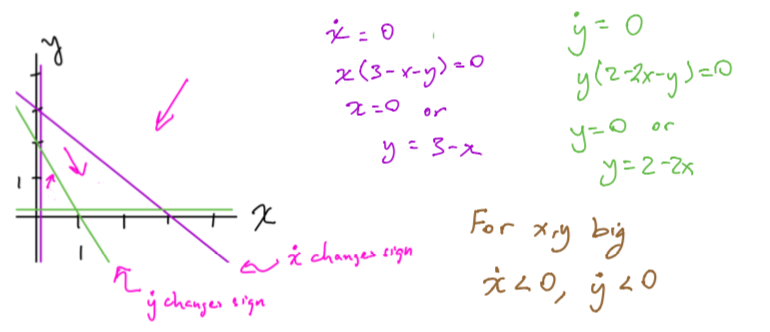
\includegraphics[width=0.9\textwidth]{img/C10-11nullclines-p1.png}


\vspace{0.2cm}

\hrule
\vspace{0.2cm}

\begin{questions}


\item (6.3.6 - from Wednesday's sheet) Consider the system
$\displaystyle\begin{array}{c c c}
 \dot{x} = & f(x,y) = x y - 1 \\
 \dot{y} = & g(x,y) = x - y^3
\end{array}$
 \begin{parts}
 \item Use \textbf{substitution} to show that $(-1,-1)$ and $(1,1)$ are both fixed points of the system (i.e. is $f(x,y) = 0$ and $g(x,y) = 0$ at these points?).  
 
 Determine whether there are other fixed points.
 \item Use Taylor polynomials to approximate the dynamical system to second order about the fixed point $(-1, -1)$.  
 
 Let $u = x-(-1)$, $v = y - (-1)$ and use this to simplify your expressions.
 
 \emph{I am asking you to approximate to second order as a review of Taylor approximation.}
 
 \begin{tcolorbox}
 
 Extra notes on Taylor polynomials:
 
 When we find a linear approximation (a first order Taylor polynomial) to a function at a point $Q$ we are identifying a linear function that has the same value as the function of interest at $Q$ and that has the same first derivatives as the original function at $Q$.
 
 When we construct a higher order approximation, of order $p$  (a $p$th order Taylor polynomial), we are finding a function such that the first $p$ derivatives match between the approximation and the original function at $Q$.
 
It may be helpful to recall that
 \begin{align*} 
 f(x,y) \approx& f(a,b) + (x-a)f_x(a,b) + (y-b) f_y(a,b) + (x-a)^2\frac{f_{xx}(a,b)}{2}\\
 &+(x-a)(y-b)f_{xy}(a,b) + (y-b)^2\frac{f_{yy}(a,b)}{2} + h.o.t.
 \end{align*}

\end{tcolorbox}
\item Sufficiently close to $(-1,-1)$, we have $\vert u \vert, \vert v\vert \ll 1$ and $u^2 \ll \vert u \vert, v^2 \ll \vert v \vert,$ so quadratic order and higher terms are small relative to the linear terms.  

\emph{Notation note: $\ll$ is read as `much less than'.  If you'd like to read a discussion of its meaning, see}

\small{\url{https://math.stackexchange.com/questions/1516976/much-less-than-what-does-that-mean#1516998}}
\begin{itemize}
\item Drop these higher order terms to generate a linearization of the system.  
\item Use your linearization to write a dynamical system of the form \[\dot{\underline{u}} = A \underline{u},\] giving definitions for $\underline{u}, A$. \\
\item Explain why the linearization leads to this kind of matrix equation only at a fixed point.  What would be the form of the linearized system away from a fixed point?
\end{itemize}

\item Create a linearized system about the fixed point $(1,1)$ as well.
\item Classify your fixed points as  \textbf{hyperbolic} (\emph{no eigenvalues have zero real part}) or \textbf{nonhyperbolic} 
 (\emph{at least one eigenvalue has zero real part}) fixed points.  \\ 
 
 \emph{Since $\Delta = \lambda_1\lambda_2$, there is a zero eigenvalue when $\Delta = 0$.  If $\tau = 0$ there may be a complex conjugate pair of eigenvalues with zero real part, the eigenvalues might both be real and sum to zero, or the eigenvalues might both be zero.  In the case of a c.c. pair with zero real part, find the sign of the determinant.} \\
 
The Hartman-Grobman theorem tells us that stability information from the linearization can be used to classify hyperbolic fixed points.  When a fixed point is nonhyperbolic the stability information from linearization is not so useful.
 \\

Identify the stability of any hyperbolic fixed points.  (Classify them as attracting, repelling, or saddle points, and identify whether they are stable or unstable).
 
  \item Use eigenvalues and eigenvectors to sketch neighboring trajectories to the two fixed points.  Try to fill in the rest of the phase portrait.  \\
  
  What do you think the long term behavior would be for a trajectory starting at $(2,2)$?  What about for one starting at $(1,2)$?

 \end{parts}
 
\item (6.4.2) Consider the system $\dot x = x(3-2x-y), \dot y = y(2-x-y)$, $x,y\geq 0$.
\begin{parts}
\item Find the fixed points.
\item Draw the nullclines on the $xy$-plane.
\item Compute the Jacobian matrix.
\item Classify the fixed points.
\end{parts}

\end{questions}

\eject


%For what conditions on $\lambda_1$ and $\lambda_2$ (and thus on $\tau$ and $\Delta$) would all solutions eventually approach the fixed point at $\underline{x} = \underline{0}$?

\eject 
\textbf{Answers:}
\begin{questions}
    
    

\question 
\begin{parts}
\item no others that are real.  
\item $\dot{u} = -u-v+uv, \dot{v} = u-3v+3v^2$.  
\item $\underline{u} = \left(\begin{array}{c} u \\ v \end{array}\right)$, $A = \left(\begin{array}{c c }-1 & -1 \\ 1 & -3 \end{array}\right)$.  
\item $\dot{u} = u+v, \dot{v} = u - 3v$. \item  both are hyperbolic.  stable f.p. at $(-1,-1)$ and unstable f.p. at $(1,1)$.  \item phase portrait is below.  Starting at $(2,2)$ it looks like we would go out the unstable manifold of the saddle point towards the right.  Starting at $(1,2)$ it looks like we will approach the stable fixed point.

\end{parts}

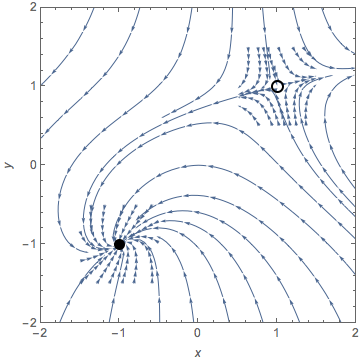
\includegraphics[width=3in]{img/Act19-02-20C08p1.png}

\end{questions}

\end{document}